\section{A Synthesized and Refined View of Assurances} \label{sec:synthesis}
    \edit{BRING IN SOME MATERIAL FROM LIPTON, GUNNING, WELLER, AND DOSHI-VELEZ}
    From the review of Quadrants I. through IV. of the formal/informal, explicit/implicit plane, we are able to find some insights with respect to assurances and can discuss them in a more comprehensive way. Using insights from the survey a refined version of Figure~\ref{fig:SimpleTrust_one_way} can be constructed. Figure~\ref{fig:refined_assurances} incorporates all details from Section~\ref{sec:background} as well as adding some insights from the survey that give direction about the design of assurances in human-AIA trust relationships. 
   
   Below we synthesize and discuss the design of explicit assurances in this more detailed framework -- some of these insights might also apply to implicit assurances, but implicit assurances will not be directly discussed in this paper.

    \begin{figure}[htbp]
        \centering
        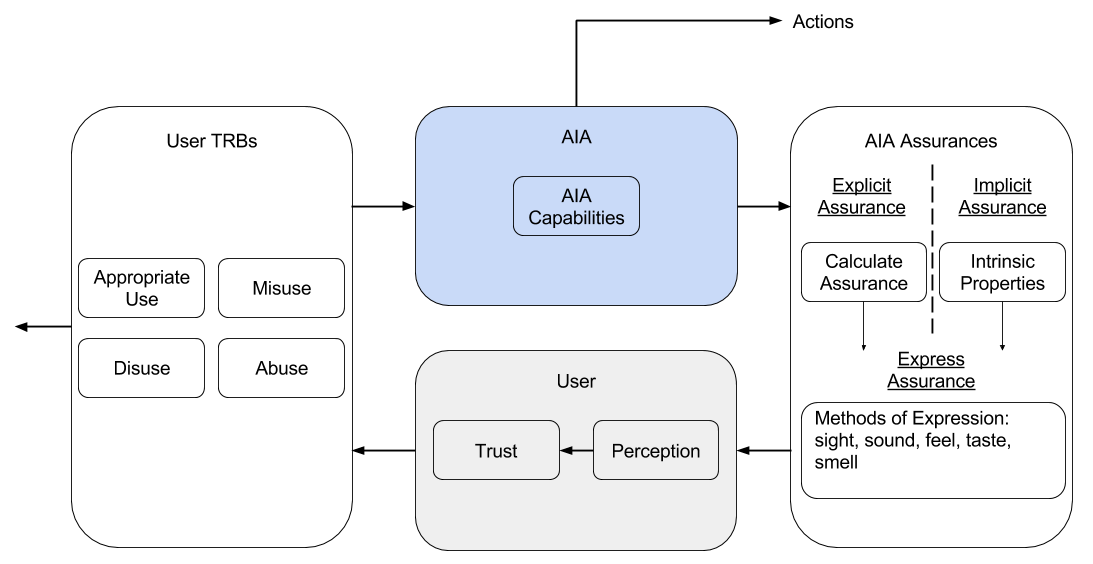
\includegraphics[width=0.9\textwidth]{Figures/RefinedTrust_one_way}
        \caption{Detailed extension of Figure~\ref{fig:SimpleTrust_one_way}. The AIA, User , and User TRBs blocks are defined as discussed in Section~\ref{sec:background} (with the exception of the `Perception' blocks added to the AIA and User boxes). The AIA Assurances box has been filled using insights from the surveyed material. The boxes that are greyed out will not be discussed in this section.}
        \label{fig:refined_assurances}
    \end{figure}

\subsection{Calculating, Designing, and Planning Explicit Assurances}
    Recall that an assurance is defined as \emph{any} behavior or property of an AIA that affects a user's trust, therefore an explicit assurance is any assurance that was consciously implemented/applied by the designer before deployment of the AIA with the express intention of influencing a user's TRB/trust (whether or not the means for doing so conforms to a formal trust concept). As such, it is possible to design assuring properties into the system a priori. It is likewise possible to design assuring behaviors into an AIA. From the literature, there are some high-level ideas that surround the calculation of assurances: 

    \begin{itemize}
        \item Quantifying Uncertainty
        \item Reducing Complexity
        \item Assurance by Design
        \item Planning Strategies of Assurance
    \end{itemize}

    \paragraph{Quantifying Uncertainty} Being able to quantify the different kinds of uncertainty in the AIA is necessary before attempting to express that uncertainty to a human user. There are several different kinds of uncertainty that might be considered such as uncertainty in sensing, uncertainty in planning, and uncertainty in locomotion. The general idea is that a model or method needs to be incorporated in the AIA that will represent the different kinds of uncertainty to the human user in some way. A human user could use such information to inform their trust in the `situational normality', `competence', and/or `predictability' of the AIA. 

    In the surveyed literature we have seen the following main approaches to do this. In some cases uncertainty is already represented intrinsically by the algorithms and/or models being used in the AIA. Some use the built-in statistical representations of transitions and observations as the basis of quantifying uncertainty in a POMDP robot. This is an approach that has straightforward analogs in systems that use algorithms and/or models that inherently consider uncertainty.

    Models and methods that intrinsically contain or represent uncertainty are frequently available. However, even when that it is the case -- such as with POMDPs featuring transition probabilities and observation probabilities -- there are types of uncertainties that may still not be considered. For example, there are further metrics of uncertainty beyond those intrinsically captured by a planner \cite{Aitken2016-fb,Kuter2012-bv}. Using the UGV road-network problem as an example, if the UGV calculates a distribution over possible outcomes, how favorable is that distribution? Or, given a certain road-network what kind of accuracy can be expected from the POMDP solver that the UGV is equipped with? Generally these considerations might be described as addressing `uncertainties in application', which are those uncertainties that arise when trying to apply certain algorithms and models in various environments.

    Perhaps the most obvious (but not necessarily simple) approach is to quantify the uncertainty of a classifier, i.e. its probability of error in making a decision (regression methods have analogous approaches). Some have approached this problem by using a GP model for classification \cite{Gurau2016-hs}. In this way they, in essence, construct a model from empirical training data and used that model to quantify uncertainty in different test scenarios. In contrast, we might quantify the uncertainty of a classifier based solely on the input itself \cite{Zhang2014-he}. Of course these methods share common drawbacks of being solely supervised learning approaches, however even in the unsupervised domain such as reinforcement learning, methods for avoiding highly uncertain (un-safe) rewards use some form of external expert knowledge (see \cite{Garcia2015-rs, Lipton2016-dq}). 

    Uncertainty can be easier to assess if some kind of oracle, or reference is available for comparison. Quantifying the similarity between the empirical experience and the available reference can be a measure of uncertainty \cite{Kaipa2015-hy}. Of course this approach loses its appeal when a truth model isn't available. This shouldn't detract from the intent of finding some kind of reference (truth or otherwise) in which the reasoning, sensing, and other processes of an AIA can be compared to evaluate uncertainty. The evaluation of statistical models involves a very similar concept: given a statistical model as a reference does current empirical experience support or detract from the hypothesis that the model is still valid \cite{Laskey1995-jp,Ghosh2016-dl}? These approaches can quantify the degree to which the statistical models are still true, and this measurement can be used as an indication of uncertainty.

    Generally, the capability of quantifying uncertainty enables an AIA to be able to express assurances related to the `situational normality', `competence', and `predictability' of the system in a given situation. One might imagine that, in the UGV road-network problem, the UGV expressing high uncertainty in its plan would influence the competence component of the user's trust. Conversely, if an uncertainty measure is not available the user might take this as an implicit assurance that the AIA is perfectly confident, or based on the user's experience they might conclude that since all AIA plans have been flawed in the past, the plan of this AIA must be flawed as well.

    \paragraph{Reducing Complexity} Many researchers have attempted to remove complexity from the models and logic of the AIA to make the methods more interpretable (or comprehensible, or explainable, \ldots) to a human user. As with quantifying uncertainty, making an AIA more interpretable can also inform a user's trust regarding the `situational normality', `competence', and `predictability' of it. Of course this presupposes that many of the methods used by AIAs are `complex' by some measure, we claim that the fact that experts are required to understand some of the methods (and even then it may not be totally possible) proves this supposition. Complexity only exists in the presence of some reference frame, which is the designer's in this case. Generally complexity is said to increase with the number of variables, steps of reasoning, the size of data, etcetera.

    In practice, reduction of complexity has been addressed by approaches as simple as finding summary statistics, or calculating averages \cite{Muir1994-ow,Muir1996-gt}. This can also be accomplished by computing heuristic measures which reduce many complex goals into more manageable pieces\cite{Aitken2016-fb}. Creating variable fidelity models is another way by which complexity can be reduced (and increased when necessary). Attempts should be made to make/discover/learn models with scalable interpretability based on given criteria like required depth of understanding, level of expertise, and time to gain understanding.
    
    One might focus on creating and using models that are inherently more interpretable to humans (i.e. \cite{Caruana2015-za} and others). This could include constraining the feature space to be more simple, reducing dimensionality, learning more understandable features, and theoretically founding the models (i.e. interpretable science).
    
    While it is possible that there are inherently interpretable models that can be designed that can compete with other non-interpretable models, we believe that this is not the best long-term approach to reducing complexity; this is primarily due to the lack of scalability for engineers and scientists to frequently design new algorithms. Investigating methods that generate explanations from non-interpretable models is a more promising direction. The main reason is that the idea of interpretable models is not well-defined and, in reality, doesn't exist as a single tangible goal. Instead there is a continuum of interpretability that is based on the complexity of the problem, the time required for a user to interpret (i.e. a few seconds or months of study), the expertise of the user, and others. Investigating the generation of interpretations and explanations that are user specific and model agnostic would be the best of both worlds. These ideas are much more aligned with the efforts of \cite{Ruping2006-xj} and others who seek to use models with scalable resolution and accuracy.

    \paragraph{Assurance by Design} No matter how much engineers like to think about automating everything, realistically a human will need to be involved at some level of assurance design for the foreseeable future, if only because the main pursuit of human-AIA trust directly involves a human. The above two approaches alone (quantifying uncertainty, and reducing complexity) can largely use existing methods, however some researchers directly engineered their methods and models in the AIA to be more meaningful to humans.

    One approach is putting a human in the learning process, which essentially modifies the objective function of the learning algorithm \cite{Freitas2006-qo}. In essence the objective function would then be based on a large set of human preferences (and biases). This kind of approach is promising, in that it can be used to encode many human qualities that cannot be easily quantified, or even explained. However, there are trade-offs that can be undesirable in many situations as well. We often use designed, objective, learning algorithms \emph{to avoid} human biases. It is interesting to note that using a human in the loop can offer more interpretability to the result of a learning process, while at the same time making the learning process itself less procedural.

    One source of discord between what humans expect and what AIAs actually do (i.e. less predictable AIAs) is a poorly designed objective function \cite{Amodei2016-xi}. This might be referred to as myopic objectives, when an AIA focuses on a specific objective to the extent that a human can no longer relate to the objective of the AIA (and will be correspondingly surprised by its actions). This suggests that significant time may be required to design objectives that align with those of humans, this alignment will automatically make the AIA more predictable, and competent in the user's eyes.

    It is also possible to modify standard learning approaches (like the ones discussed in the previous section), in such a way as to make the methods inherently more assuring to a human. For example one might restructure a neural net architecture, or a decision tree with the sole purpose of making it more interpretable \cite{Choi2016-by,Abdollahi2016-vn,Jovanovic2016-gw}. It is difficult however, because it is not always clear how this can/should be done.

    \paragraph{Planning Explicit Assurances} Planning assurances is critical when trying to attain desired TRBs from a human user. In this context when we say `planning explicit assurances' we mean formulating a plan for the expression of assurances over time, with the goal of more effectively and appropriately expressing assurances to a human user. Having said this we recognize that planning is not a capability available to all AIAs. In cases where AIAs don't have the ability to plan, they may be designed beforehand with some kind of static plan of assurance. Otherwise, more advanced AIAs might take into account TRBs to plan an assurance strategy to assist the human to use it appropriately.

    When planning assurances the AIA must be able to account for limitations of users, and its own limitations in expressing assurances. For example a user may not be able to understand the necessary information needed to use the AIA more appropriately. Also, the AIA may need to take a long-term strategy to teach the user, as opposed to only presenting the user with canned, static, assurances. Some of the important user considerations will be discussed further in Section~\ref{sec:express_assurances}.
    
    One must ask whether the human user can correctly process the information received. This is perhaps most easily illustrated by considering a non-expert user who cannot understand highly technical assurances regarding the AIA. However, less trivial manifestations may be troubling, such as the existence of bias in the perception of assurances. This will be addressed further in Section~\ref{sec:express_assurances}.

    This topic is nearly unexplored in the context of human-AIA trust relationships. However, there are several fairly new programs that are interested in this question (i.e. explainable artificial intelligence (XAI) \cite{Gunning2016-kb}, and assured autonomy \cite{Neema2017-bb}). Assuming an AIA can give assurances there are important questions like: what is the best way to present them? How can they be adapted for different kinds of users? How can the AIA teach or tutor the human over time? This is a large gap in the current assurances landscape, answers to these questions are critical to designing more robust and effective assurances.

\subsection{Expression and Perception of Assurances} \label{sec:express_assurances}
    Expression and Perception of assurances have been combined in this section because they share several critical aspects. The key points to be considered in design of assurances are:
    
    \begin{itemize}
        \item Mediums
        \item Methods
        \item Efficacy
    \end{itemize}
    
    For an explicit assurance the medium, and method of expression must be selected taking into consideration the limitations of the AIA. Here medium denotes the means by which an assurances is expressed, this could be through any of the senses by which humans perceive, such as sight, sound, touch, smell, and taste. The method of assurance is the way by which the assurance is expressed. An example may help: a plot may be conveyed through sight in the typical way, or through spoken language (for example when communicating to a blind person); in this case the plot is the method, and sight or sound are the different mediums through which it can be communicated. An AIA might be limited in methods of expression because it does not have a display, or a speaker. In that situation how is the user supposed to receive an assurance?

    A designer must also consider whether a human can perceive the assurances being given. If so, to what extent is the information from the assurance transfered, or how efficacious was the assurance? A few examples include: an AIA giving an auditory assurance in a noisy room and the user not hearing it (such as an alert bell in a factory where the workers use ear-plugs), or an AIA attempting to display an assurance to a user that has obstructed vision. If an assurance is not expressed, or not perceived by the user, it is useless and has no effect. For example, an AIA may have the ability to store data about its performance, and compute a statistic regarding its reliability, but if it cannot successfully express (or communicate) that information in some way, the information is useless.

    A user will \emph{always} have some kind of TRB towards an AIA (if only to choose to ignore the AIA). In the absence of explicit assurances the human will instead use implicit assurances to inform their TRBs. However, the general human user will not have knowledge regarding which assurances are implicit or explicit -- humans participating in research from Quadrants I and II were not aware which assurances were designed by the researchers and which weren't. Recall from Section~\ref{sec:assurances} that to a user all assurances are the same; that is to say that any property or behavior of an AIA that affects trust is an assurance to a user, and it doesn't matter whether the assurance was designed for that purpose or not (is explicit or implicit).

    \paragraph{Mediums:} One might use sight to express an assurance. For example an AIA might give visual feedback, or display different performance characteristics \cite{Chadalavada2015-wx,Muir1996-gt}. This can also be accomplished by using natural language \cite{Wang2016-id} -- it is also a simple matter to convert written natural language output to spoken natural language now. Other typical mediums are blinking lights, colored boxes, ringing bells, buzzers, recorded voice alerts and others.
    
    The other senses (touch, smell, and taste) are not well explored in literature related to human-AIA trust. Generally, any human sense could be used as a medium. Besides sight, and sound, one of of tactile feedback has been used extensively in robotics where it is called `haptic feedback' (where the user receives mechanical feedback through the robot controls). This medium is use to create a more immersive user interface in robotics, to help users feel more connected to the robot. One can imagine smell and taste having an obvious application in the assurances of a cooking robot, other applications certainly exist as well and are open to further research.

    \paragraph{Methods:} One of the main methods by which to express an assurance is by displaying a value, such as a flow-rate \cite{Muir1996-gt}. While this may sound banal it actually involves some nuanced points. The interesting part is that a value such as a flow-rate actually conveys no assurance to a human user without the human user then creating a corresponding mental model of the trustworthiness of an AIA capability. The user's trust dimensions (`competence', 'predictability', etcetera) are then affected by this perception. This approach (also used by \cite{Wickens1999-la,Sheridan1984-kx,Hutchins2015-if} and others) is effective, but relies heavily on the assumption that the user will create a model that is `good enough' out of sequentially presenting certain information.

    Similarly one might train a user to recognize signs of failure in different interactions with an AIA \cite{Freedy2007-sg,Desai2012-rc,Salem2015-md}. Still this approach relies on human users to make models that are `good enough' in order to correctly decide how to appropriately use the AIA. The main drawback of this work, and of that above is the blind reliance on users being able to make correct statistical models (of things like reliability) from noisy observations. A more ideal approach would be to design assurances that remove chances for misinterpretation because of inconsistent human models.

    More direct methods of expressing assurances include displaying the intended movements through visual projection of a planned path \cite{Chadalavada2015-wx} -- this is subtly, but significantly different from making the user infer the intended intention. Analogously, natural language expressions (written or otherwise) attempt a more active method of expressing an assurance (such as \cite{Wang2016-id}). One might also display plans and logic in different formats such as tables or trees, bar charts  \cite{Van_Belle2013-ph, Huysmans2011-th, Hutchins2015-if}. These approaches attempt to remove some uncertainty regarding the human's ability to create the correct model. As humans are fond of saying ``You can't assume that I can read your mind!'', in essence more passive expressions from AIAs are relying on humans to read AIA's `minds' (we can't even do that with other humans).

    Any of these methods can be more or less effective based on the task, or situation in which they are used. How should uncertainly be displayed (i.e. as a distribution, summary statistics, fractions or decimals)?  Unsurprisingly we find that the answer is `it depends' \cite{Chen2014-dk,Wallace2001-fm,Kuhn1997-qc,Lacave2002-cu}. Things such as the experience of the user, or the nature of the information being displayed affect the user's ability to interpret the assurance. In the absence of that information the best that can be done is to select the method that will work for the largest group of typical users of the AIA. A sufficiently advanced AIA might also be able to learn the best methods to communicate to different users on a one-on-one basis.

    It is generally presumed that making something more human-like will make an AIA more trustworthy. An algorithm may be human-like when it represents knowledge in a way that a human would understand, or executes logic in a way that a human can follow. A robot that is humanoid becomes more human-like in appearance \cite{Bainbridge2011-pl}, a system that uses natural language becomes more human-like in communication \cite{Lacave2002-cu}. The human-AIA trust relationship depends on assurances that, in essence, are conversions from AIA capabilities to human-perceptible behaviors and properties.  Assurances are the method of communication upon which humans can learn to trust AIAs. Because of this it is expected that at some point all assurances have to at least be made human-understandable in some way, otherwise the AIA is essentially speaking a different language, and assurances cannot be understood.

    Making something `human-like' doesn't always increase it's trustworthiness. In \cite{Dragan2013-wd} the AIA is made more trustworthy by making the robot motions more human-like, whereas in \cite{Wu2016-ei} making the AIA more human-like resulted in a decrease of trustworthiness. In this case the difference came from the type of task, in the first case the robot was physically working in proximity to a human, in the other case the user was playing a competitive game against the AIA. It has been observed that humans trust more `human-like' AIAs in more human-like ways \citet{Tripp2011-rx}. Perhaps `human-like' applies to how difficult it is to relate to the AIA. Following on this idea the benefits or drawbacks of human-like characteristics are influenced by a user's general impressions and feelings of how trustworthy humans are in similar situations. This would also involve aspects of psychology, sociology, and is very difficult to control and account for. This is an open research question that is important to answer in order to design better assurances.

    It is worth considering, in more detail, what implications the existence of implicit and explicit assurances has on the designer. It is unrealistic to think that a designer can take all possible assurances into account, and thus will need to focus efforts on some of the most important. The foremost consideration is that an analysis of the interaction between the human and user needs to be made in order to identify the critical assurances for a given scenario. For example, in the road network problem, an analysis might find that the most critical assurances are about the competence of the UGV's planner. In this case the designer must take time to design an assurance that is directed at the user's perception of the AIA's competence -- let's call this a planning-competence assurance.

    One difficulty arises from this approach is that there doesn't seem to be a way to determine what passive assurances might drown out active assurances. Following from the example above, the designer may have built an excellent planning-competence assurance, but failed to consider the effect of how the UGV appears -- it may be old, have loose panels, and rust holes. Generally, designers overlook implicit assurances (i.e. do not consider them explicitly in design) because they assume that they will have no effect (i.e. why does it matter if there are rust-holes if the UGV works?). This can stem from either: 1) ignorance of human-AIA trust dynamics, or 2) lack of identifying which assurances are most important to a human user.

    While it might be nice, it seems unreasonable, inefficient, and unwise to attempt a study of \emph{every possible} assurance from an AIA to a human and then select the most important. Perhaps one way a designer might try to identify which assurances are important is to perform human studies where feedback about which characteristics of the AIA most affected the trust of the user. An approach like this would help to point out if explicit assurances are being noticed, and if there are implicit assurances that are overly influential, or that overwhelm the explicitly designed assurances. With such feedback designers would have a realistic idea about whether their explicit assurances are having the desired effect. We use the UGV road-network problem to illustrate. After designing an explicit assurance (or more) the operator/UGV team could work together, afterwards the operator could rank the different behaviors/properties of the AIA affected their trust in it. In this way the critical implicit and explicit assurances will be identified. If the explicit assurance is near the top of the list of influencing assurances then it is working, if not a re-design may need to occur.

    One final point is that there are several potential sources of explicit assurance that lack appropriate expressions, and thus cannot be effectively utilized as assurances. For example, it is unclear the best way for an AIA to express that it has been validated and verified on situations similar to the current one. Similarly, what other methods exist for communicating statistical distributions besides showing a plot (only useful for 1 or 2 dimensional distributions) or showing sufficient statistics? Investigating how assurances can be expressed in effective, and efficient ways is critical to human-AIA trust relationships.

    \paragraph{Efficacy:} Some kinds of expression are very `one-dimensional' in that they only use one medium, or method. This, again, has been seen in practice by the utilization of plotting a certain value over time. Because of this, much of the research to date involves assurances that are not robust to loss in transfer, meaning that the approaches count everything on a specific medium and method to work, and if not the whole assurance is rendered useless. Hence, exploring ways in which assurances can be robustly communicated is a clear opportunity for those trying to design assurances. This is akin to a human speaking with their voice, making facial expressions, and gestures with their hands as well; simultaneously utilizing several mediums/methods helps to ensure an assurance will be effective. Of course, repeating the same message over a thousand times is wasteful, and so enters the idea of efficiency in expression.

    Perhaps less obvious is a situation in which the user has to supplement an incomplete assurance. A user can supposedly create a mental model of the trustworthiness of an AIA capability -- based on repeated observations over time. Creating this mental model takes time, and the model is prone to cognitive biases. In this case the assurance is communicated slowly and indirectly. Generally, a highly effective assurance would have precise information communicated in a way that is easy for the user to perceive, with little loss. Whereas, an inefficient, and ineffective assurance may be more vague, wasteful (i.e. repeating the same thing a thousand times), and susceptible to loss in communication. The solutions to efficacy lay in selecting appropriate methods, and mediums for expression of the assurance, and by designing for appropriate levels of redundancy to ensure that the assurance is received.

\subsection{Observing Effects of Assurances} \label{sec:measuring_effects}

    Since the purpose of assurances is to affect TRBs, it is important to be able to quantify those effect. There are two different instances in which this is useful: 1) when the designer needs an understanding of how effective the assurances are; and 2) When the  AIA needs to observe the efficacy of it's own assurances.
    
    To our knowledge there has not been any work regarding the second situation that enables an AIA to observe responses to assurances and then adapt behaviors appropriately (at least not in the trust cycle setting), however this is arguably the ultimate goal so that AIAs can themselves modify assurances to meet different needs. What does this mean practically? Theoretically, any method that is made for the designer to measure the effects of assurances could also be deployed into an AIA. The surveyed literature gives some insights into how that has been done to date.
   
    When it comes time to measure the effect of assurances on a human's trust there are two main approaches:
    
    \begin{itemize}
        \item Gather self-reported changes in trust from human users
        \item Measure changes in user's TRBs
    \end{itemize}
    
    \paragraph{Self-Reported Changes} Gathering self-reported changes in trust involves asking questions like: `how trustworthy do you feel the system is?'; or `to what extent do you find the system to be interpretable?' \cite{Mcknight2011-gv,Muir1996-gt,Wickens1999-la,Salem2015-md,Kaniarasu2013-ho}. These kinds of questions can be useful in verifying whether the assurances are having the expected effect. It is not unreasonable to imagine that an AIA might be equipped with a method by which it can ask the user questions about their trust, process those responses, and modify assurances appropriately.
    
    However, sometimes changes is self-reported trust do not result in changes in TRBs \cite{Dzindolet2003-ts}. From the AIAs perspective this means that --- unless the object of the assurances is to make the person's level of self-reported trust change --- the assurances are not providing any benefit. As previously discussed, the goal of assurances is to elicit appropriate TRBs from the human user. From this perspective, measuring changes in TRBs is the more direct, and objective, approach to measure the effect of assurances.

    Self-reports are the most useful when trying to understand the true effects of an assurance. Does a certain assurance, assumed to affect `situational normality', actually do that? There is space for quite a lot of research in this realm. Does displaying a specific plot actually convey information about `predictability'? This information can be used to inform the selection of the methods of assurance.

    \paragraph{Measuring Changes in TRBs} Generally researchers in the field have measured, in some way, how frequently the AIA was able to run in autonomous mode before being turned off \cite{Freedy2007-sg,Desai2012-rc}. Other researchers calculated whether the user was willing to cooperate with the AIA or not \cite{Salem2015-md,Wu2016-ei,Bainbridge2011-pl}. A better defined metric is: the likelihood of appropriate use of a certain capability by the user; albeit more difficult to formally define/calculate in different situations. As a concrete example, in the UGV road-network problem there isn't really an option to `turn off' the UGV. Instead the remote operator can make decisions such as accepting a plan designed by the UGV. In this situation the effect of assurances might be measured by how likely the operator is to accept a generated plan instead of overriding it (recall that the goal may not be to have the generated plan accepted 100\% of the time, rather that it be accepted with respect to how appropriate it is in a given situation).

    In practical application (such as in the UGV road-network problem), the user, and the human-AIA team, care more about whether TRBs are appropriate or not. It doesn't help if an assurance helps the user feel that the AIA is more competent, if the user doesn't treat the AIA any differently than before the assurance. This assumes that it is possible for appropriate TRBs to be measured in the first place. For example, if appropriate behavior is for the user to verify a sensor reading, can the AIA perceive that happening? In that situation perhaps the easiest approach would be to ask the user, but what if the user is dishonest? Is there a way to verify the user behavior is actually appropriate? This is something that has gained notoriety with the current generation of autonomous cars, where the car is capable of autonomous operation, but the user still needs to sit in the driver's seat and be attentive just in case the vehicle cannot perform correctly. These are some arguments for the importance of designing methods for perceiving appropriate (and inappropriate) TRBs when designing assurances. 
%
% \subsection{The Imprecise Nature of Assurances} \label{sec:imprecise_nature}
    % Due to the nature of trust (and humans in general), a single assurance might be targeted at influencing the competence dimension of trust, but it may also have effects on other dimensions. As an example an assurance that targets predictability may also have an affect on the probability of depending.
%
    % Besides being difficult to separate effects on a single user, individual users are different as well. Thus no assurance will have an identical effect when given to two separate users. This makes it difficult to have precise effects on user trust behaviors.
%
    % One might attempt to mitigate this uncertainty by using expressions that are more precise than others, such as displaying a probability distribution rather than on a maximum likelihood. This gets into some considerations about how the presentation of information affects the ability of a human to understand.
